\section{Method}

Given a natural language prompt, PEC-Nav extracts a structured navigation goal, explores using a self-calibrating frontier search, stores observations in episodic memory, and answers follow-up questions from that memory. Figure~\ref{fig:architecture} gives an overview.

\begin{figure*}[t]
\centering
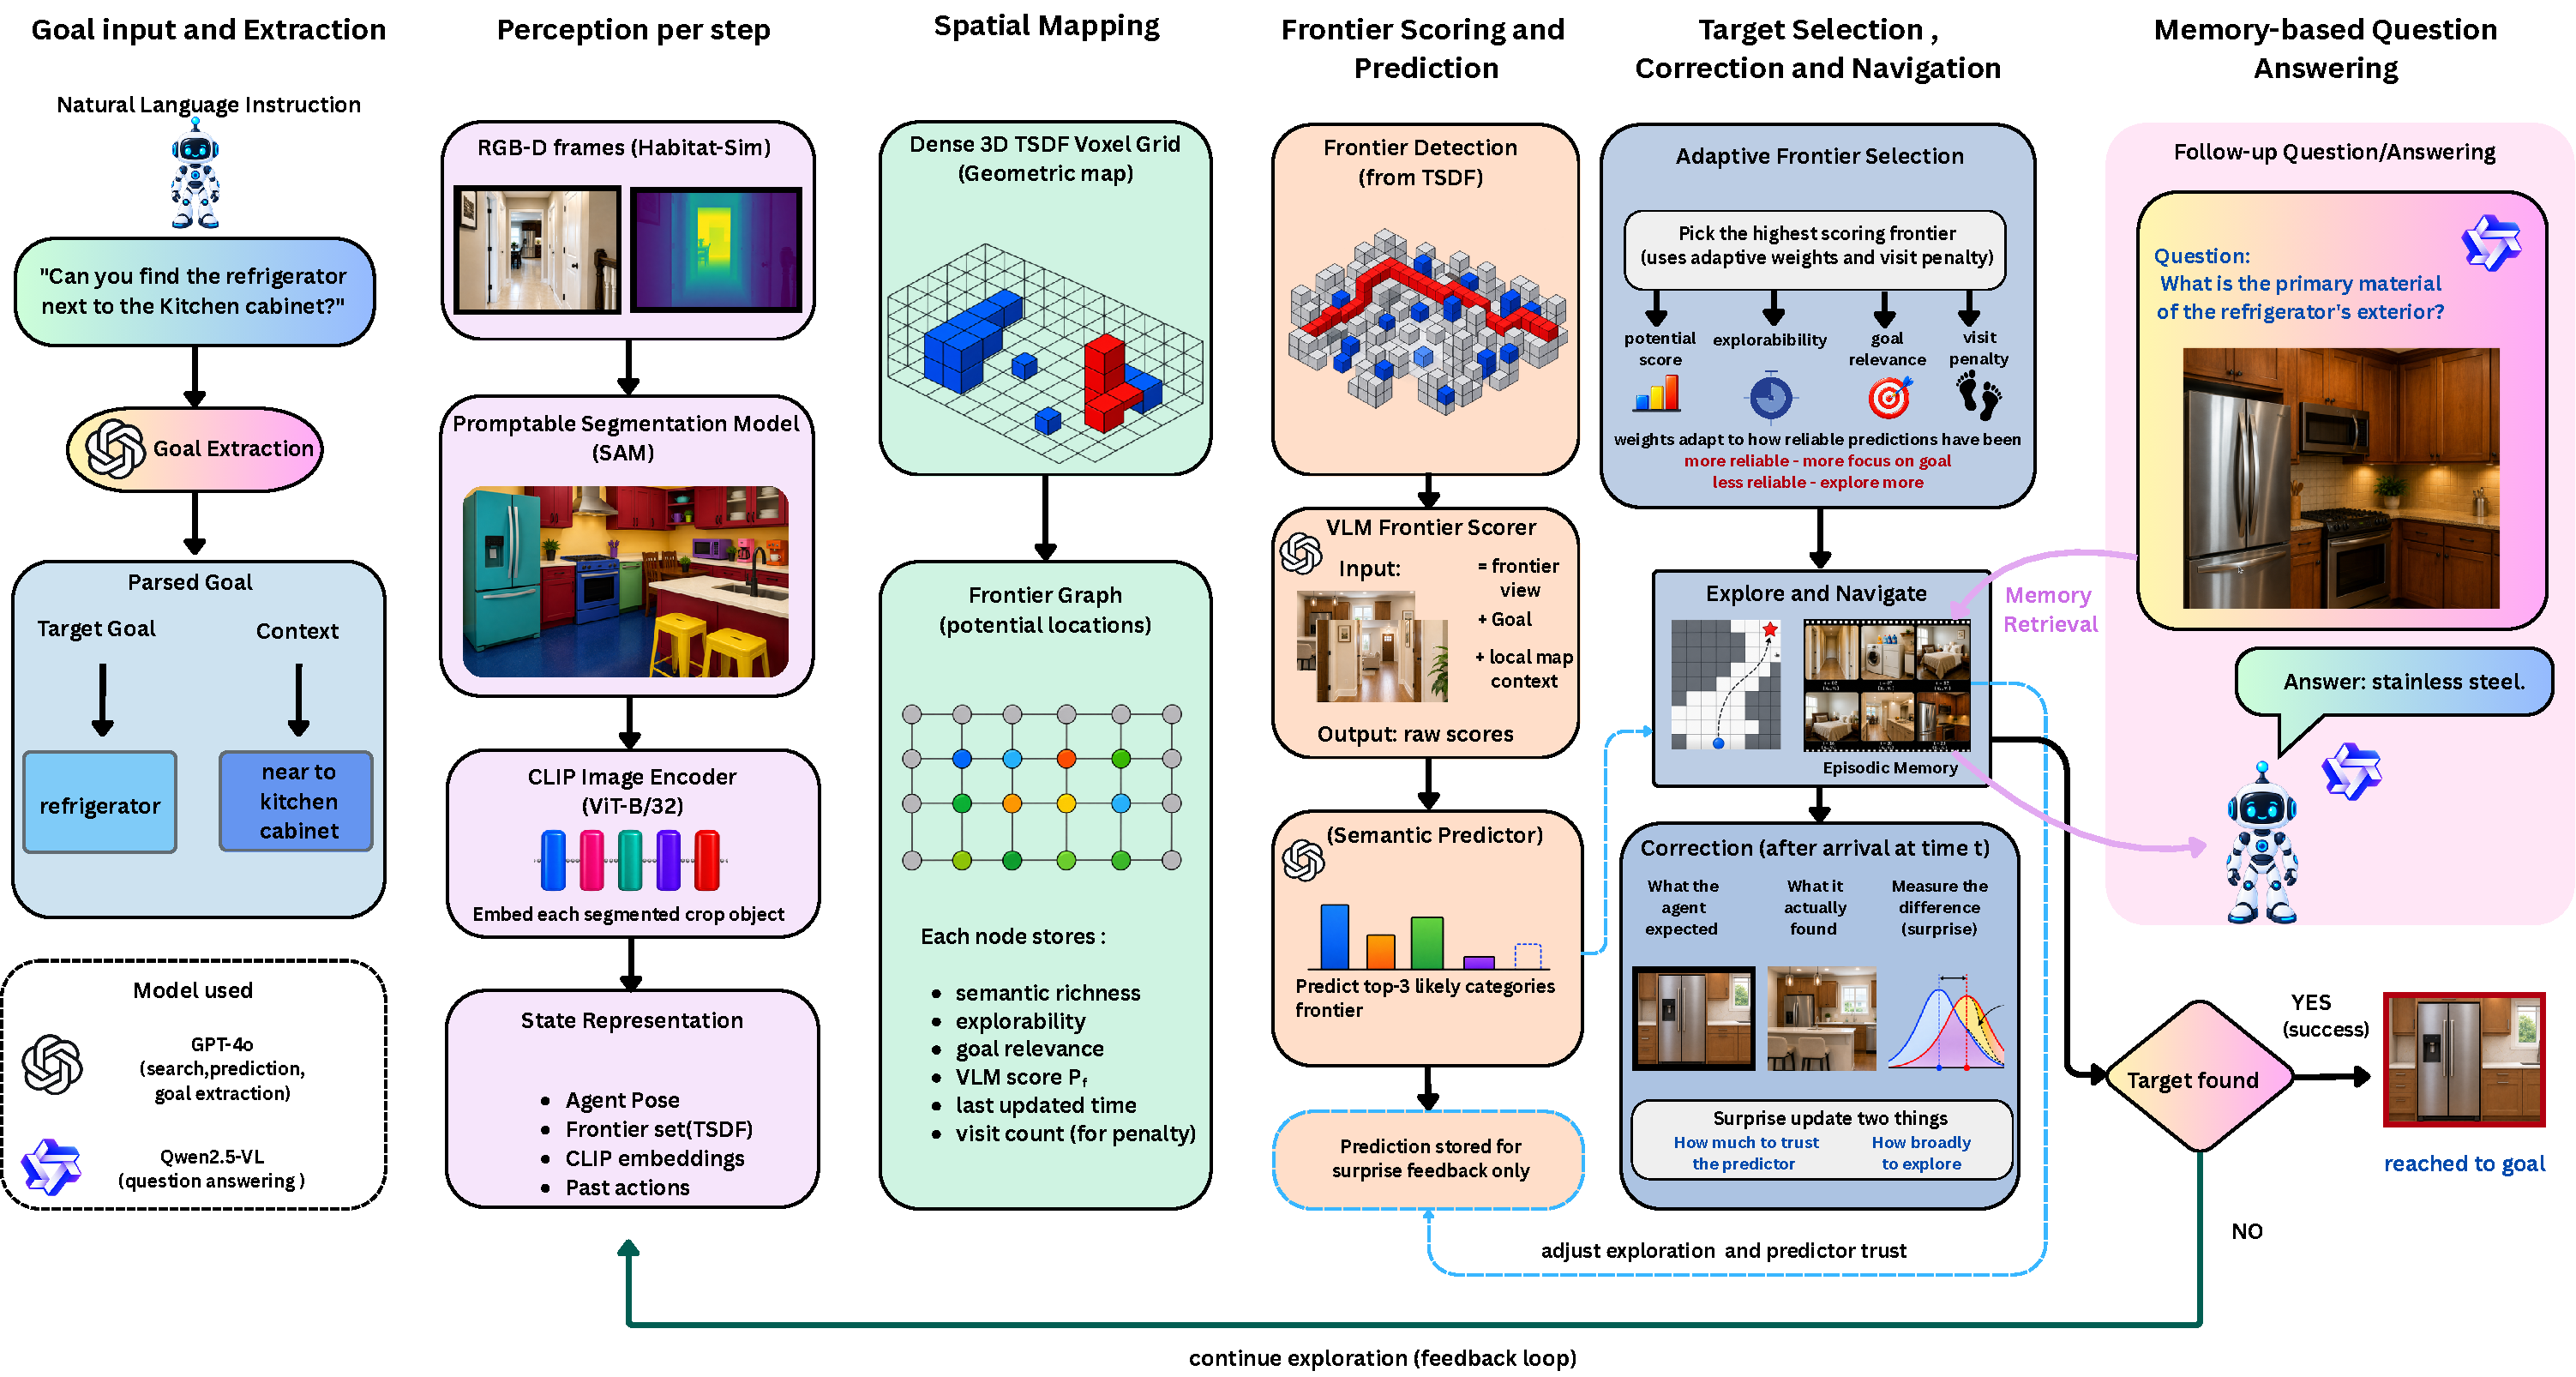
\includegraphics[width=0.93\textwidth]{figures/Pec-main-architecture .pdf}
\caption{\textbf{Illustration of PEC-Nav.} The agent predicts the layout beyond each frontier, selects one, explores it, and corrects the predictor on arrival, and can answer follow-up questions using the episodic memory populated during exploration.}
\label{fig:architecture}
\end{figure*}

\subsection{Goal Extraction}
\label{sec:problem}

Unlike standard ObjectNav, where the goal is a category label or image, our agent receives a natural language prompt such as \emph{``Can you find the refrigerator next to the kitchen cabinet?''}, which carries both spatial context and relational cues. We extract a structured goal using GPT-4o~\cite{openai2024gpt4o}, which receives only the prompt text, with no scene geometry or ground-truth labels, and outputs a \textbf{target category} such as ``refrigerator'' and a \textbf{contextual description} such as ``likely in a kitchen, near cabinets''. This structured goal drives both frontier scoring and semantic prediction throughout the episode.

\subsection{Predict-Explore-Correct Loop}
\label{sec:pec}

The agent fuses egocentric RGB-Depth (RGB-D) observations into a TSDF voxel grid, from which it derives a top-down occupancy map and identifies frontiers as boundaries between explored and unexplored space. Object proposals come from a promptable segmentation model (SAM) and are embedded with a CLIP image encoder~\cite{radford2021clip}, giving the sparse semantic graph over which frontiers are scored. The agent scores each frontier $f$ with a VLM that produces semantic richness ($r_f$), explorability ($e_f$), goal relevance ($g_{r,f}$) and a potential estimate ($p_f$). The four are separate VLM outputs rather than a summary and its parts, and the value function of Sec.~\ref{sec:calibration} uses three of them, with $r_f$ entering only as context for the prompt that produces $p_f$. A frontier scored at step $t'$ and reconsidered at step $t$ carries its score forward discounted by $\gamma^{\,t - t'}$ with $\gamma = 0.95$, so stale assessments lose weight relative to fresh ones. This scoring follows the formulation surveyed in Sec.~\ref{sec:related-frontier} and is not what we contribute, beyond computing goal relevance against our text goal rather than a reference image.

Our contribution is the loop closed around that scorer. One design property is worth stating first. The prediction $\hat{P}_f$ is never a term in $\mathrm{val}(f)$, and its only route into behaviour is the surprise it generates on arrival, which sets $\sigma_t$ and the weights scoring subsequent frontiers. The semantic predictor shapes search by being wrong in a measurable way rather than by voting on the next move.

\paragraph{Prediction.} For each frontier the VLM is prompted with the frontier's egocentric view and the extracted goal, returning the top-3 categories $\{c_1, c_2, c_3\}$ with confidences $\hat{p}_i \in [0,1]$. These are modulated by a self-calibration scale $\sigma_t \in (0.4, 1.0]$ (set by Eq.~\ref{eq:adapt}) and normalised over $C = \{c_1, c_2, c_3, \text{other}\}$,
\begin{align}
    u(c_i) &= \hat{p}_i \, \sigma_t, \quad
    u(\text{other}) = \max\!\left(\epsilon,\, 1 - \textstyle\sum_{i=1}^{3} \hat{p}_i \, \sigma_t\right)
    \label{eq:predict} \\
    \hat{P}(c) &= u(c) \big/ \textstyle\sum_{c' \in C} u(c') . \notag
\end{align}
Normalisation is required rather than cosmetic, since the three confidences need not sum to one and the $\max$ flooring the residual mass can push the total past it. The constant $\epsilon = 10^{-3}$ prevents zero probabilities and also smooths the counts in Eq.~\ref{eq:observed}, regularising both distributions identically. The effect of $\sigma_t$ survives normalisation, since as it falls, mass transfers into the \emph{other} bucket and the agent becomes less committed. Each $\hat{P}_f$ is keyed by the frontier's voxel position and view and scored on arrival as issued rather than rescaled, so surprise measures the error of the belief the agent acted on.

\paragraph{Exploration.} The agent selects $f^* = \arg\max_f \mathrm{val}'(f)$ (Eq.~\ref{eq:calibrate}--\ref{eq:visitpenalty}) and navigates toward it with a point-goal controller, recording egocentric RGB observations into an episodic memory buffer with spatial-temporal coordinates.

\paragraph{Correction.} When the agent comes within $R = 3.0$\,m of a previously predicted frontier, correction fires. The distance is taken on the $(x,z)$ ground plane after transforming the agent's position from the simulator frame to the map frame,
\begin{equation}
    d = \left\lVert \big(w_f^{(x)}, w_f^{(z)}\big) - \big(\mathrm{pts}_{\text{norm}}^{(x)}, \mathrm{pts}_{\text{norm}}^{(z)}\big) \right\rVert_2 ,
    \label{eq:arrival}
\end{equation}
where $w_f$ is the frontier's stored world-frame position and $\mathrm{pts}_{\text{norm}}$ the agent's position after that transform. It then builds an observed distribution over the same support,
\begin{equation}
    Q(c) = \frac{\mathrm{count}(c) + \epsilon}{\sum_{c' \in C} \big(\mathrm{count}(c') + \epsilon\big)} .
    \label{eq:observed}
\end{equation}
These counts come from the Habitat simulator's semantic sensor, so correction consumes privileged information a deployed agent would obtain from a detector, and the accuracy of $Q$ upper-bounds what a detector-based variant would supply. Predict, explore and goal extraction use no ground-truth labels. Restricting both distributions to this small prediction-specific support is what makes the comparison informative, since over a full vocabulary the observation would be near one-hot and the divergence would measure vocabulary sparsity instead of predictive error. The surprise signal is
\begin{equation}
    D_{\mathrm{KL}}(\hat{P} \,\|\, Q) = \sum_{c \in C} \hat{P}(c) \log \frac{\hat{P}(c)}{Q(c)} ,
    \label{eq:kl}
\end{equation}
which is bounded, since flooring both arguments at $\epsilon$ caps any single term at $\log(1/\epsilon) \approx 6.9$ nats. A confident prediction that is fully contradicted therefore produces a large but finite surprise, keeping the signal at the $O(1)$ magnitude the squash below expects.

\subsection{Self-Calibration}
\label{sec:calibration}

Surprise drives two feedback paths through a shared running estimate. We maintain an EMA of per-correction values and squash it to a bounded signal,
\begin{equation}
    \bar{s}_t = (1 - \beta)\,\bar{s}_{t-1} + \beta \, D_{\mathrm{KL}}^{(t)}, \quad
    n_t = 1 - e^{-\bar{s}_t} ,
    \label{eq:ema}
\end{equation}
with $\beta = 0.3$ and $\bar{s}_0 = 0$, an optimistic prior under which the agent trusts its predictions until evidence accumulates. The first path, \textsc{correct-confidence}, scales the predictor's confidence,
\begin{equation}
    \sigma_t = 1 - 0.6\, n_t \in (0.4, 1.0] .
    \label{eq:adapt}
\end{equation}
The regime this produces matters for reading our results. The map is strongly compressive above $\bar{s} \approx 2$, where every value sends $n_t$ into $[0.86, 1)$ and $\sigma_t$ into $(0.4, 0.48]$, so it discriminates sharply among small surprises and barely among large ones, and with $\beta = 0.3$ the EMA reaches it within roughly five corrections. The intent is fast commitment rather than gradual annealing, with the floor bounding how far distrust can go.


\begin{table*}[htbp]
\centering
\caption{\textbf{Results on LMEE-Bench.} Upper block is retrieval-augmented QA over memory banks collected post-exploration, lower block is active exploration.}
\label{tab:lmee}
\footnotesize
\setlength{\tabcolsep}{3pt}
% \begin{tabular}{lcccccccccccccccc}
\begin{tabular}{l|cccc|cccc|cccc|cccc}

\toprule
& \multicolumn{4}{|c}{\textbf{Easy}} & \multicolumn{4}{|c}{\textbf{Medium}} & \multicolumn{4}{|c}{\textbf{Hard}} & \multicolumn{4}{|c}{\textbf{Total}} \\
\cmidrule(lr){2-5} \cmidrule(lr){6-9} \cmidrule(lr){10-13} \cmidrule(lr){14-17}
& \multicolumn{2}{c}{Nav} & \multicolumn{2}{c|}{QA} & \multicolumn{2}{c}{Nav} & \multicolumn{2}{c|}{QA} & \multicolumn{2}{c}{Nav} & \multicolumn{2}{c|}{QA} & \multicolumn{2}{c}{Nav} & \multicolumn{2}{c}{QA} \\
\cmidrule(lr){2-3} \cmidrule(lr){4-5} \cmidrule(lr){6-7} \cmidrule(lr){8-9} \cmidrule(lr){10-11} \cmidrule(lr){12-13} \cmidrule(lr){14-15} \cmidrule(lr){16-17}
\textbf{Method} & SR & SPL & Score & Acc & SR & SPL & Score & Acc & SR & SPL & Score & Acc & SR & SPL & Score & Acc \\
\midrule
\multicolumn{17}{l}{\emph{Retrieval-Augmented QA}} \\
LLaVA-OneVision-7B~\cite{li2024llavaov} & N/A & N/A & 35.71 & 57.14 & N/A & N/A & 42.02 & 62.77 & N/A & N/A & 25.00 & 43.75 & N/A & N/A & 38.62 & 59.31 \\
Llama3.2-Vision-11B & N/A & N/A & 43.57 & 48.57 & N/A & N/A & 28.19 & 37.23 & N/A & N/A & 20.31 & 31.25 & N/A & N/A & 31.03 & 39.31 \\
Qwen2.5-VL-7B & N/A & N/A & 36.43 & 65.71 & N/A & N/A & 43.62 & 53.19 & N/A & N/A & 42.19 & 43.75 & N/A & N/A & 41.72 & 55.17 \\
InternVL3-8B & N/A & N/A & 42.14 & 65.71 & N/A & N/A & 41.22 & 54.26 & N/A & N/A & 26.56 & 43.75 & N/A & N/A & 39.83 & 55.86 \\
Qwen3-VL-8B~\cite{bai2025qwen3} & N/A & N/A & 43.57 & 65.71 & N/A & N/A & 36.70 & 58.51 & N/A & N/A & 32.81 & 62.50 & N/A & N/A & 37.93 & 60.69 \\
GPT-4o~\cite{openai2024gpt4o} & N/A & N/A & 43.57 & 65.71 & N/A & N/A & 37.50 & 51.06 & N/A & N/A & 40.62 & 56.25 & N/A & N/A & 39.31 & 55.17 \\
Gemini-2.5-Flash & N/A & N/A & 44.29 & 51.43 & N/A & N/A & 37.77 & 50.00 & N/A & N/A & 23.44 & 50.00 & N/A & N/A & 37.76 & 50.34 \\
\midrule
\multicolumn{17}{l}{\emph{MLLM Exploration}} \\
Explore-EQA~\cite{ren2024exploreeqa} & 4.26 & 4.26 & N/A & N/A & 15.17 & 8.67 & N/A & N/A & 14.89 & 7.25 & N/A & N/A & 13.24 & 7.66 & N/A & N/A \\
3D-Mem~\cite{huang20243dmem} & 21.28 & 9.68 & 30.71 & 42.86 & 15.73 & 6.09 & 34.57 & 44.68 & 17.02 & 6.97 & 25.00 & 18.75 & 16.91 & 6.86 & 32.59 & 41.38 \\
RA-Mem$^{\ddagger}$~\cite{wang2026memoryexplorer} & 25.53 & 15.65 & 34.29 & 54.29 & \textbf{21.35} & 12.14 & 37.77 & 62.77 & 14.89 & 8.86 & 25.00 & 43.75 & 20.96 & 12.18 & 35.52 & 58.62 \\
MemoryExplorer~\cite{wang2026memoryexplorer} & 31.91 & 21.11 & 35.71 & \textbf{68.57} & \textbf{21.35} & 14.03 & 48.14 & 63.83 & 23.40 & 12.51 & 34.38 & \textbf{68.75} & 23.53 & 14.99 & 43.62 & 65.52 \\
\midrule
\textbf{PEC-Nav (Ours)} & \textbf{40.43} & \textbf{25.06} & \textbf{48.57} & \textbf{68.57} & 20.11 & \textbf{14.35} & \textbf{62.77} & \textbf{67.02} & \textbf{25.00} & \textbf{18.21} & \textbf{50.00} & 56.25 & \textbf{24.45} & \textbf{16.86} & \textbf{57.93} & \textbf{66.21} \\
\bottomrule
\end{tabular}
\end{table*}

The second path, \textsc{correct-weights}, shifts the value function along the explore-exploit spectrum,
\begin{align}
    \mathrm{val}(f) &= w_p \, p_f + w_e \, e_f + w_g \, g_{r,f} \label{eq:calibrate} \\
    w_p &= 0.5, \quad w_e = 0.3 + 0.2\,n_t, \quad w_g = 0.2 - 0.2\,n_t , \notag
\end{align}
with weights summing to one for all $n_t$. Under sustained surprise $w_e$ reaches 0.5 and $w_g$ falls to zero, so selection is carried by how much unexplored potential a frontier offers rather than by how well it matches the goal. This makes $w_g$ the most aggressively scheduled term, and whether a nonzero floor on it would serve better is untested. A soft visit penalty then discourages unproductive revisitation,
\begin{equation}
    \mathrm{val}'(f) = \mathrm{val}(f) \cdot \max\!\left(0.1, \; \frac{1}{1 + 0.5 \cdot \mathrm{visits}(f)}\right) ,
    \label{eq:visitpenalty}
\end{equation}
where the floor of 0.1 keeps repeatedly visited frontiers from being scored out entirely.

Algorithm~\ref{alg:pecnav} summarises the decision cycle.

\begin{algorithm}[htbp]
\caption{PEC-Nav decision cycle}
\label{alg:pecnav}
\begin{algorithmic}[1]
\REQUIRE Frontiers $\mathcal{F}$, goal $g$, state $(\sigma_t, n_t, \bar{s}_t)$
\ENSURE Selected frontier $f^*$, updated state
\FOR{each $f \in \mathcal{F}$}
    \STATE $p_f, e_f, g_{r,f} \leftarrow \text{VLMScore}(f, g)$
    \STATE $\hat{P}_f \leftarrow \text{PredictLayout}(f, g, \sigma_t)$ \COMMENT{Eq.~\ref{eq:predict}, stored not scored}
    \STATE $\mathrm{val}'(f) \leftarrow$ Eq.~\ref{eq:calibrate}--\ref{eq:visitpenalty}
\ENDFOR
\STATE $f^* \leftarrow \arg\max_{f} \mathrm{val}'(f)$, navigate toward $f^*$
\IF{$d(f') \le R$ for any previously-predicted $f'$}
    \STATE $Q \leftarrow \text{ObservedLayout}(f')$ \COMMENT{Eq.~\ref{eq:observed}}
    \STATE $\bar{s}_t \leftarrow (1{-}\beta)\bar{s}_{t-1} + \beta \, D_{\mathrm{KL}}(\hat{P}_{f'} \| Q)$
    \STATE $n_t \leftarrow 1 - e^{-\bar{s}_t}$, \quad $\sigma_t \leftarrow 1 - 0.6 n_t$, \quad update $w_e, w_g$
\ENDIF
\end{algorithmic}
\end{algorithm}

\subsection{Memory, QA and Implementation}
\label{sec:memory}

Every egocentric RGB observation is stored with spatial-temporal coordinates, and follow-up questions are answered by retrieving and reasoning over them. Across our ablations memory and QA are held identical with only search varying, so changes in answer quality there are attributable to search. This does not extend to the published rows of Table~\ref{tab:lmee}, whose memory modules differ.

Question answering runs locally on a Qwen2.5-VL-7B model, with the full protocol in Sec.~\ref{sec:setup}. Table~\ref{tab:hyperparams} lists all hyperparameters, tuned on 5 development scenes and then fixed.

\begin{table}[htbp]
\centering
\caption{PEC-Nav hyperparameters. $\dagger$ marks an inherited default.}
\label{tab:hyperparams}
\footnotesize
\setlength{\tabcolsep}{4pt}
\begin{tabular}{@{}llll@{}}
\toprule
\textbf{Symbol} & \textbf{Value} & \textbf{Symbol} & \textbf{Value} \\
\midrule
$\gamma^\dagger$ & 0.95 & $w_p$ & 0.5 (fixed) \\
$\epsilon$ & $10^{-3}$ & $w_e$ & $[0.3, 0.5]$ \\
$R$ & 3.0\,m & $w_g$ & $[0.0, 0.2]$ \\
$\beta$ & 0.3 & $\sigma_t$ & $(0.4, 1.0]$ \\
$\bar{s}_0$ & 0 & Visit disc., floor & 0.5,\; 0.1 \\
\bottomrule
\end{tabular}
\end{table}

